\chapter{York Extensible Testing Infrastructure}
\label{chap:yeti_3}

%\section{Random Testing}


%%%%%%%%%%%%%%%%%%%%%%%%%%%%%%%%%%%%%%%%%%%%%%
%													        %
%														 %			
% YETI Section Starts here									 %
%														 %		
%														 %
%%%%%%%%%%%%%%%%%%%%%%%%%%%%%%%%%%%%%%%%%%%%%%

\section{YETI Overview}
York Extensible Testing Infrastructure (YETI), an automated random testing tool developed in Java, is capable of testing programs written in Java, JML and .NET languages~\cite{Oriol2010c}. YETI takes program byte code as input and execute it with random generated but syntactically-correct inputs to find a fault. It runs at a high level of performance with $10^6$ calls per minute on Java code. One of its prominent feature is Graphical User Interface (GUI), which make YETI user friendly and provides option to change testing process in real time. It can also distribute large testing tasks in cloud for parallel execution~\cite{Oriol2010}. The latest version of YETI can be downloaded from \url{https://code.google.com/p/yeti-test/downloads/list}. Figure \ref{fig:yetiOverview} briefly presents the working process of YETI. 
\begin{figure}[h]
	\centering
	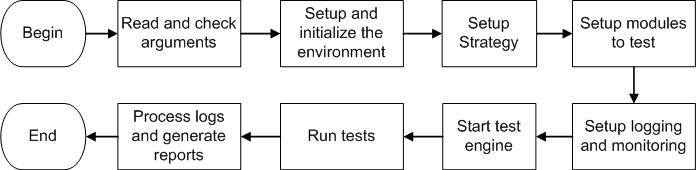
\includegraphics[width=15cm, height=4.5cm]{chapter3/yetiOverview.png}
	\caption{Working process of YETI}
	\label{fig:yetiOverview}
\end{figure}


\subsection{YETI Design}
YETI has been designed with the provision of extensibility for future growth. YETI enforces strong decoupling between test strategies and the actual language constructs, which adds new binding, without any modification in the available test strategies. YETI can be divided into three main parts on the basis of functionality: the core infrastructure, the strategy and the language-specific binding. Each part is briefly described below. 

\subsubsection{Core Infrastructure}
The core infrastructure is responsible for test data generation, test process management and test report generation. The core infrastructure is split into four packages: yeti, yeti.environments, yeti.monitoring, yeti.strategies. The package yeti uses classes from yeti.monitoring and yeti.strategies packages and calls classes in the yeti.environment package as shown in the Figure \ref{fig:yetiCore}. 

\begin{figure}[h]
	\centering
	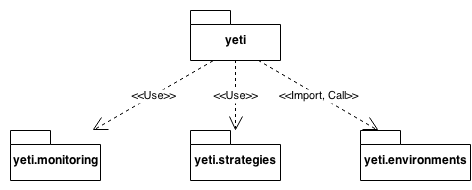
\includegraphics[width=15cm, height=7cm]{chapter3/yetiCore.png}
	\caption{Main packages of YETI with dependencies }
	\label{fig:yetiCore}
\end{figure}

The most essential classes included in the YETI core infrastructure are:
\begin{enumerate}
\item {\textbf{Yeti:}} It is the entry point to YETI and contains the main method. It parses the arguments, sets up the environment, initializes the testing and delivers the reports of the test results.
\item {\textbf{YetiLog:}} It prints debugging and testing logs. 
\item {\textbf{YetiLogProcessor:}} It is an interface for processing testing logs.
\item {\textbf{YetiEngine:}} It binds YetiStrategy and YetiTestManager together, which carry out the actual testing process.
\item {\textbf{YetiTestManager:}} It makes the actual calls based on the YetiEngine configuration, activate the YetiStrategy to generate test data and select the routines.
\item {\textbf{YetiProgrammingLanguageProperties class:}} It is a place holder for all language related instances.
\item {\textbf{YetiInitializer:}} It is an abstract class for test initialization.
\end{enumerate}

\subsubsection{Strategy}
The strategy defines a specific way to generate test inputs. This part contains six essential strategies stated below.
\begin{enumerate}
\item {\textbf{YetiStrategy:}} It is an abstract class which provides interface for every strategy in YETI.
\item {\textbf{YetiRandomStrategy:}} It implements the random strategy and generates random values for testing. The strategy gives choice to the user to adjust null values probability and the percentage of creating new objects for the test session. 
\item {\textbf{YetiRandomPlusStrategy:}} It extends the random strategy by adding interesting values to the list of test values. The strategy gives the choice to the user to select the percentage of interesting values used in the test session.
\item {\textbf{DSSRStrategy:}} It extends random+ strategy by adding the values surrounding the fault value. The strategy is described in detail in Chapter~\ref{chap:DSSR}.
\item {\textbf{ADFDStrategy:}} It extends random+ strategy by adding the feature of graphical representation of faults and their domains. The strategy is described in detail in Chapter~\ref{chap:ADFD}.
\item {\textbf{YetiRandomDecreasingStrategy:}} It extends the random+ strategy by setting the probability value to starts at 100\% and ends at 0\% when the test finishes.
\item {\textbf{YetiRandomPeriodicStrategy:}} It extends random+ strategy by setting the probability in such a way that it decreases and increases randomly during test session.
\end{enumerate}

\subsubsection{Language-specific Binding}
The language-specific binding facilitates modelling of programming languages. It is extended to provide support for a new language in YETI. The language-specific binding includes the following classes:
\begin{enumerate}
\item {\textbf{YetiVariable:}} It is a sub-class of YetiCard, which represents a variable in YETI.
\item {\textbf{YetiType:}} It represents type of data in YETI, e.g. integer, float, double, long, boolean and char.
\item {\textbf{YetiRoutine:}} It represents constructor, method and function in YETI. It has a specific name, a return type and a   It is a super type of routines which represents functions, methods and constructors. A routine is given a name, return type and list of arguments.
\item {\textbf{YetiModule:}} It represents a module in YETI and stores one or more routines of the module.
\item {\textbf{YetiName:}} It represents a unique name assigned to each instance of YetiRoutine.
\item {\textbf{YetiCard:}} It represents a wildcard or a variable in YETI, having a specific type and name.
\item {\textbf{YetiIdentifier:}} It represents an identifier for an instance of a YetiCard.
\end{enumerate}
% if java binding example is required or instead of adding new steps if you want to show only java binding then for material check the msc thesis page 40 of test c code with Yeti.

\subsection{Construction of Test Cases}
YETI construct test cases by creating objects of the classes under test and randomly calls methods with random inputs according to the parameter's-space. YETI splits input values into two types i.e. primitive data types and user defined classes. For primitive data types as methods parameters, YETI in random strategy calls $Math.random()$ method to generate arithmetic values are converted to the required type using Java cast operation. In the case of user-defined classes as a parameter YETI calls constructor or method to generate object of the class at run time. The constructor may possibly require another object, then YETI recursively calls the constructor or method of that object. This process is continued till an object with empty constructor or a constructor with only primitive types or the set level of recursion is reached.

\subsection{Command-line Options}
YETI is provided with several command line options which a tester can enable or disable according to the test requirement. These options are case insensitive and can be provided in any order as input to YETI from command line interface. As an example, a tester can use command line option $-nologs$ to bypass real time logging and save processing power by reducing overhead. Table~\ref{table:cliOptions} includes some of the common command line options available in YETI.

\begin{table}[h]
%\scriptsize
\caption{YETI command line options} % title of Table
\bigskip
\centering
{\renewcommand{\arraystretch}{1.5}
\begin{tabular}{|l|l|} % centered columns (4 columns)
\hline

Options						&Purpose 										\\ \hline
-java						&To test Java programs	 						\\ \hline
-jml							&To test JML programs							\\ \hline
-dotnet						&To test .NET programs							\\ \hline
-ea							&To check code assertions 						\\ \hline
-nTests						&To specify number of tests						\\ \hline
-time						&To specify test time								\\ \hline
-testModules				&To specify one or more modules to test 			\\ \hline
-rawlogs					&To print real time logs during test 				\\ \hline
-nologs						&To omit real time logs and print end result		\\ \hline
-yetiPath					&To specify path to the test modules				\\ \hline
-gui							&To show test session in GUI						\\ \hline
-DSSR						&To specify Dirt Spot Sweeping Random strategy 	\\ \hline
-ADFD						&To specify Automated Discovery Failure Domain strategy \\ \hline
-random					&To specify Random test strategy					\\ \hline
-randomPlus					&To specify Random plus test strategy				\\ \hline
-nullProbability				&To specify probability of inserting null values		\\ \hline
-randomPlusPeriodic			&To specify Random plus periodic test strategy		\\ \hline
-newInstanceProability		&To specify probability of inserting new objects		\\ \hline

\hline %inserts single line
\end{tabular}
}
\bigskip
\label{table:cliOptions} % is used to refer this table in the text
\end{table}


\subsection{YETI Execution}
YETI, developed in Java, is highly portable and can easily run on any operating system with Java Virtual Machine (JVM) installed. It can be executed from both CLI and GUI. To execute YETI, it is necessary to specify the $project$ and the relevant $jar$ library files, particularly $javassist.jar$ in the $CLASSPATH$. The typical command to execute YETI from CLI is given in Figure~\ref{fig:yeticommand}.

\begin{figure}[h!]
	\centering
	\frame{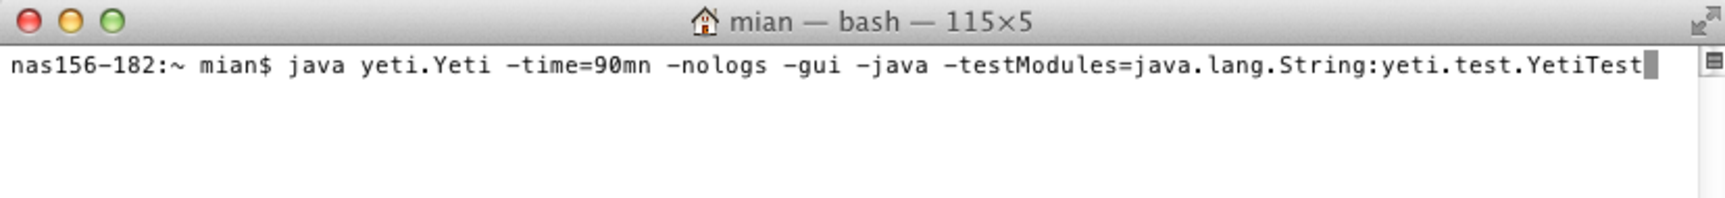
\includegraphics[width= 15cm, height = 2cm]{chapter3/yetiCommandCLI.pdf}}
	\caption{Command to launch YETI from CLI}
	\label{fig:yeticommand}
\end{figure}

 In this command YETI tests java.lang.String and yeti.test.YetiTest modules for 90 minutes using the default random strategy. Other CLI options are already indicated in Table \ref{table:cliOptions}. To execute YETI from GUI, $YetiLauncher$ presented in Figure \ref{fig:yetiLauncher} has been created for use in the present study.

\begin{figure}[h]
	\centering
	\frame{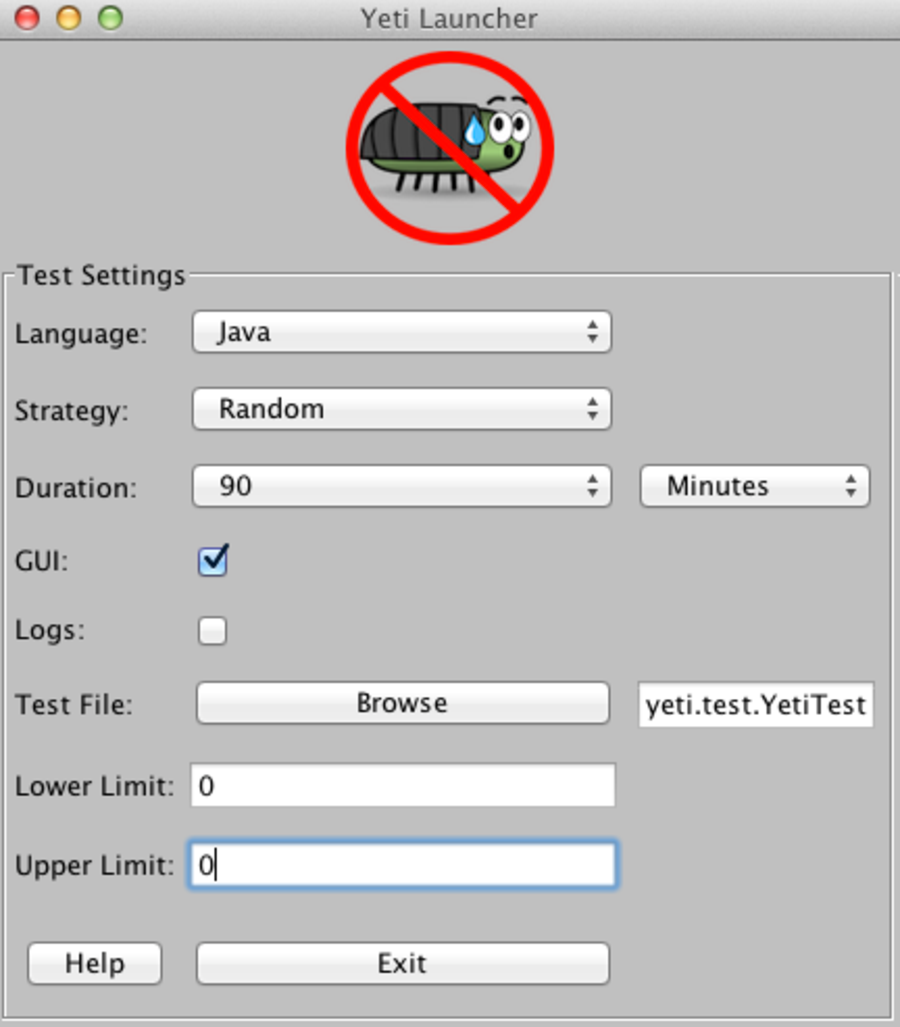
\includegraphics[width= 9.5cm, height = 11.5cm]{chapter3/yetiCommandGUI.pdf}}
	\caption{GUI launcher of YETI}
	\label{fig:yetiLauncher}
\end{figure}


\subsection{YETI Test Oracle}
YETI uses one of the two approaches for oracle. In the presence of program specifications, it checks for inconsistencies between the code and the specifications. In the absence of specifications it checks for assertion violation.% if assert statements are included by the programmer. However in the absence of 
If specifications or assertions are absent, YETI performs robustness testing which considers any undeclared runtime exceptions as failures. 

%If code contracts are available, YETI uses them as oracle, however, in their absence YETI uses undeclared runtime exceptions of the underlying language as oracle. The test cases revealing errors are reproduced at the end of each test session for unit and regression testing.
%YETI deals with the oracle problem in two ways. If available, it uses code-contracts as oracles, however in the absence of contracts it uses runtime exceptions as errors which is also known as robustness testing.

\subsection{YETI Report}
YETI gives a complete test report at the end of each test session. The report contains all the successful calls with the name of the routines and the unique identifiers for the parameters in each execution. These identifiers are recorded with the assigned values to help in debugging the identified fault. 
\\
\begin{figure}[h]
	\centering
	\frame{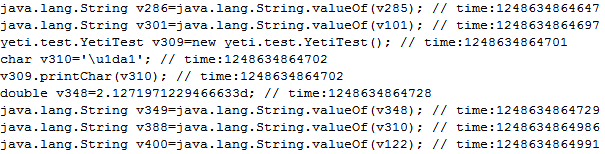
\includegraphics[width= 15cm, height = 5cm]{chapter3/yetiReport1.png}}
	\caption{Successful method calls of YETI}
\end{figure}

YETI separates the found bugs from successful executions to simplify the test report. This helps debuggers to easily track the origin of the problem rectification. When a bug is identified during testing, YETI saves the details and present it in the bug report as shown in Figure \ref{bugReport}. The information includes all identifiers of the parameters the method call had along with the time at which the exception occurs.

\begin{figure}[h]
	\centering
	\frame{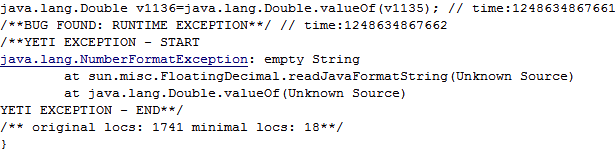
\includegraphics[width= 15cm, height = 5cm]{chapter3/yetiReport2.png}}
	\caption{A sample of YETI bug report}
	\label{bugReport}
\end{figure}

\subsection{YETI Graphical User Interface}
YETI supports a GUI that allows testers to monitor the test session and modify the characteristics in real time during test execution. It is useful to have the option of modifying the test parameters at run time and observing the test behaviour in response. Figure \ref{fig:yetiGUI1} present the YETI GUI comprising of thirteen labelled components.

\begin{figure}[h]
	\centering
	%\frame{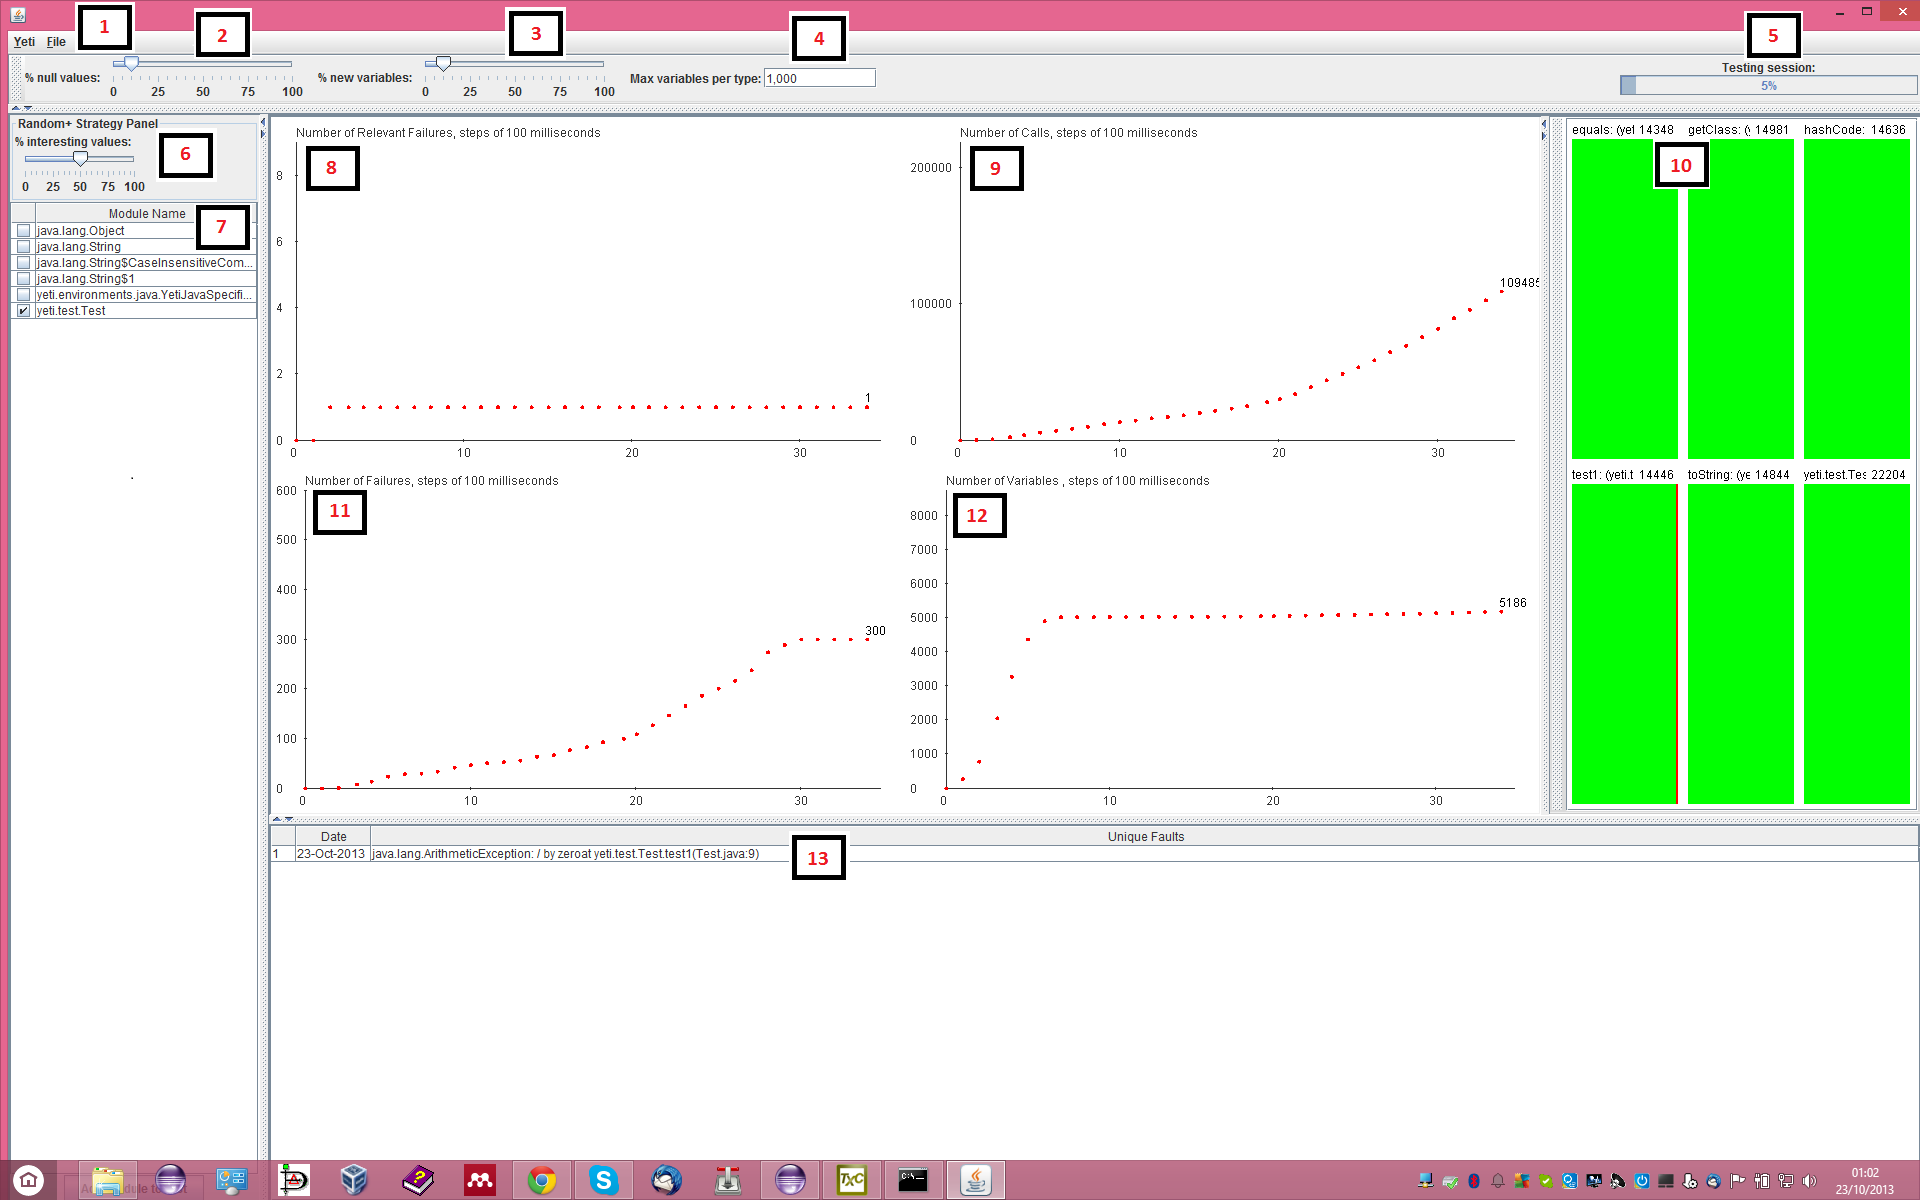
\includegraphics[width= 15cm, height = 9.8cm]{chapter3/yetiGUI.png}}
	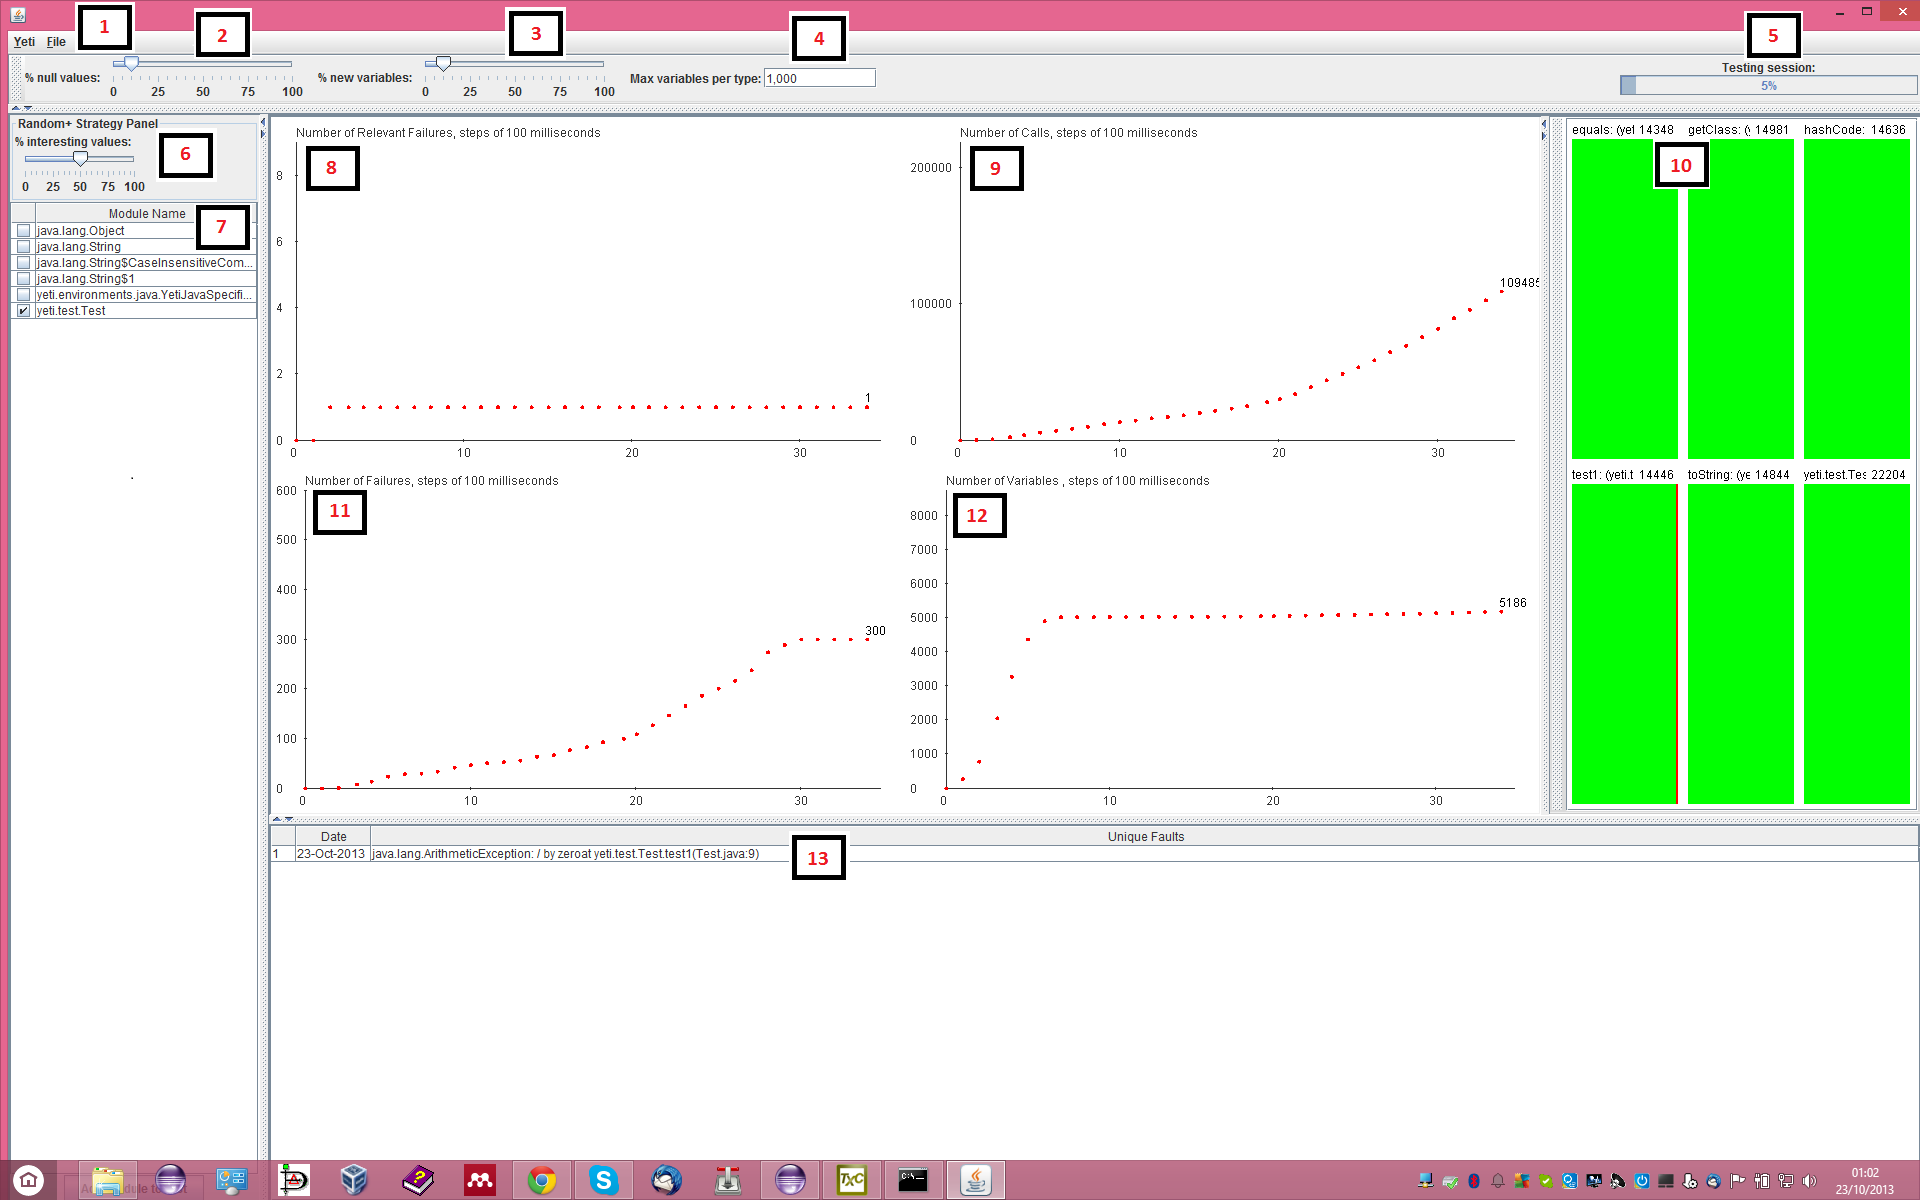
\includegraphics[width= 15cm, height = 9.8cm]{chapter3/yetiGUI.png}
	\caption{GUI of YETI}
	\label{fig:yetiGUI1}
\end{figure}

\begin{enumerate}

\item Menu bar:
\begin{enumerate}
\item Yeti menu:
\item File menu:
\end{enumerate}
\item Slider of \% null values: It displays the set probability of null values in percentage used as null instance for each variable. The default value of probability is 1. 
\item Slider of \% new variables: It displays the set probability of creating new instances at each call. The default value of probability is 1. 
\item Text-box of Max variables per type: It displays the number of variables created for a given type. The default value is 1000.
\item Progress bar of testing session: It displays the test progress in percentage.
\item Slider of strategy: It displays the set random strategy for the test session. Each strategy has its own control to change its various parameters. 
\item Module Name shows the list of the modules under the test. The
modules with ticks are the modules under test. The module names also show all the
class names in the test module.
\item Graph window 1: It displays the total number of unique failures over time in the module under test.
\item Graph window 2: It displays the total number of calls over time to the module under test.
\item Routine's progress: It displays test progress of each routine in the module represented by four colours. Mostly green and red colour appears indicating successful and unsuccessful calls respectively. Occasionally black and yellow colours appear indicating no calls and incomplete calls respectively.
\item Graph window 3: It displays the total number of failures over time in the module under test. 
\item Graph window 4: It displays the total number of variables over time generated by YETI in the test session.
%\item displays all the routines in the module under test with a rectangle.
%Each rectangle presents the results of calls of the routine. The rectangle can have in 4 colors. Black indicates no any calls of this routine. Green indicates that has successful calls of this routine. Red indicates that this routine is called unsuccessfully which means that the call to this routine results in an exception. Yellow indicates undecidable calls, for example if a call cannot finish in predefined time and Yeti stops this call, in this case yeti cannot decide this call is successful or unsuccessful. The text next the routines name show how many calls of this routine and text displays percentage of passed, failed and undescided when the cursor over the rectangle.
%\item displays a table which contains the unique faults are detected by Yeti. It records the detail of exceptions.
%\item Window No 5 displays colored rectangles: one for each constructor and method under test. Each rectangle represents the calls to a constructor or a method.
%\item The colors in a rectangle have the following meaning:
%\item Green indicates successful calls (✓). A successful call is one that does not raise an exception or if it does, the method or the constructor declares to throw it.
%\item Red indicates failed calls (X). A failed call results from raised RuntimeException or one of its subclasses.
%\item Yellow indicates “undecidable” calls (?). A call is “undecidable” if for some reason it takes too long to complete and needs to be stopped, or if a YetiSecurityException (custom exception in YETI) is thrown.
\item Report section: It displays the number of unique fault by date and time, location and type detected in the module under test. 
\end{enumerate}


\subsection{Summary}
In this chapter we define random testing and the various ways of performing random testing. We then showed how the automated testing tools implement random technique for software testing. Finally the chapter explains in detail the YETI which is being used in this study. The main features of all the tools are noted in the following table.

\begin{sidewaystable}
    \centering
    \caption{Main features of automatic testing tools used in random testing}
    \bigskip
   \begin{tabular}{|l|l|l|l|l|l|}
\hline

Tool 				& Language																								& Input  																																			& Strategy 																																											 				& Output		  																								& Benefits																															\\ \hline
JCrasher	  & Java, JML																								& Program																																			& \vtop{\hbox{\strut Method type to predict input,}\hbox{\strut Randomly find values of crash}}  				& TC																													& \vtop{\hbox{\strut Automated TC, Use} \hbox{of Heuristic Rules}} 	 \\ \hline
Jartege			& Java																										& Classes																																			& \vtop{\hbox{\strut Random strategy with controls}\hbox{\strut like weight etc.}} 							 				& TC, RT 																											& Quick, automated																									 \\ \hline
Eclat				& Java																										& Classes, pass TC 																														& \vtop{\hbox{\strut Create model from TC, execute}\hbox{\strut each candidate on the model}} 					& Faulty TC 																									& \vtop{\hbox{\strut produce output text,} \hbox{JML}}									\\ \hline
Quickcheck	& Haskell																									&	\vtop{\hbox{\strut Specifications}  \hbox{\strut and Functions}}	  			  & \vtop{\hbox{\strut Specification} \hbox{\strut hold to random TC?}} 											 						& Pass/Fail																										& \vtop{\hbox{\strut Easy to use, program} \hbox{documentation}}				\\ \hline
Randoop 		& Java, .NET																							& \vtop{\hbox{\strut Specifications,} \hbox{\strut code and time}}					  & \vtop{\hbox{\strut Generate and execute methods} \hbox{\strut \& give feedback for next generation}} 	& Fault TC, RT 																								& 																																\\ \hline
AgitarOne		& Java																										& \vtop{\hbox{\strut Package, time}   \hbox{\strut and manual TC}}						& \vtop{\hbox{\strut Analyse SUT with auto and} \hbox{\strut provided data in specified time}} 					& TC, RT																											& \vtop{\hbox{\strut Eclipse plug-in} \hbox{\& easy to use}}  			 \\ \hline
AutoTest		& Java																										& \vtop{\hbox{\strut Classes, time}   \hbox{\strut and manual TC}} 						& \vtop{\hbox{\strut Heuristic rules} \hbox{\strut to evaluate contracts}} 															& violations, RT 																							& \vtop{\hbox{\strut GUI in HTML,} \hbox{easy to use}} 								\\ \hline
TestEra			& Java																										& \vtop{\hbox{\strut Specifications,} \hbox{\strut integer \& manual TC}}			& \vtop{\hbox{\strut Check contracts} \hbox{\strut with specifications}} 																& Contracts violations 																				& \vtop{\hbox{\strut short report with} \hbox{faulty TC only}} 					\\ \hline
Korat 			& Java																										& \vtop{\hbox{\strut Specifications}  \hbox{\strut and manual tests}}					& \vtop{\hbox{\strut Check contracts} \hbox{\strut with specifications}}																& Contracts violations 																				& \vtop{\hbox{\strut GUI, short report} \hbox{with faulty TC only}} 	 \\ \hline
YETI 				& \vtop{\hbox{\strut Java, .NET,}  \hbox{\strut JML}} 		& Code, Time 																																  & RandomPlus, Random 																																										& \vtop{\hbox{\strut Traces of found } \hbox{\strut faults}}	& \vtop{\hbox{\strut GUI, give faulty} \hbox{examples, Quick}} 			 \\ \hline %inserts single line
\end{tabular}
\label{table:Tools}
\end{sidewaystable}


%\begin{figure}[h]
%	\centering
%	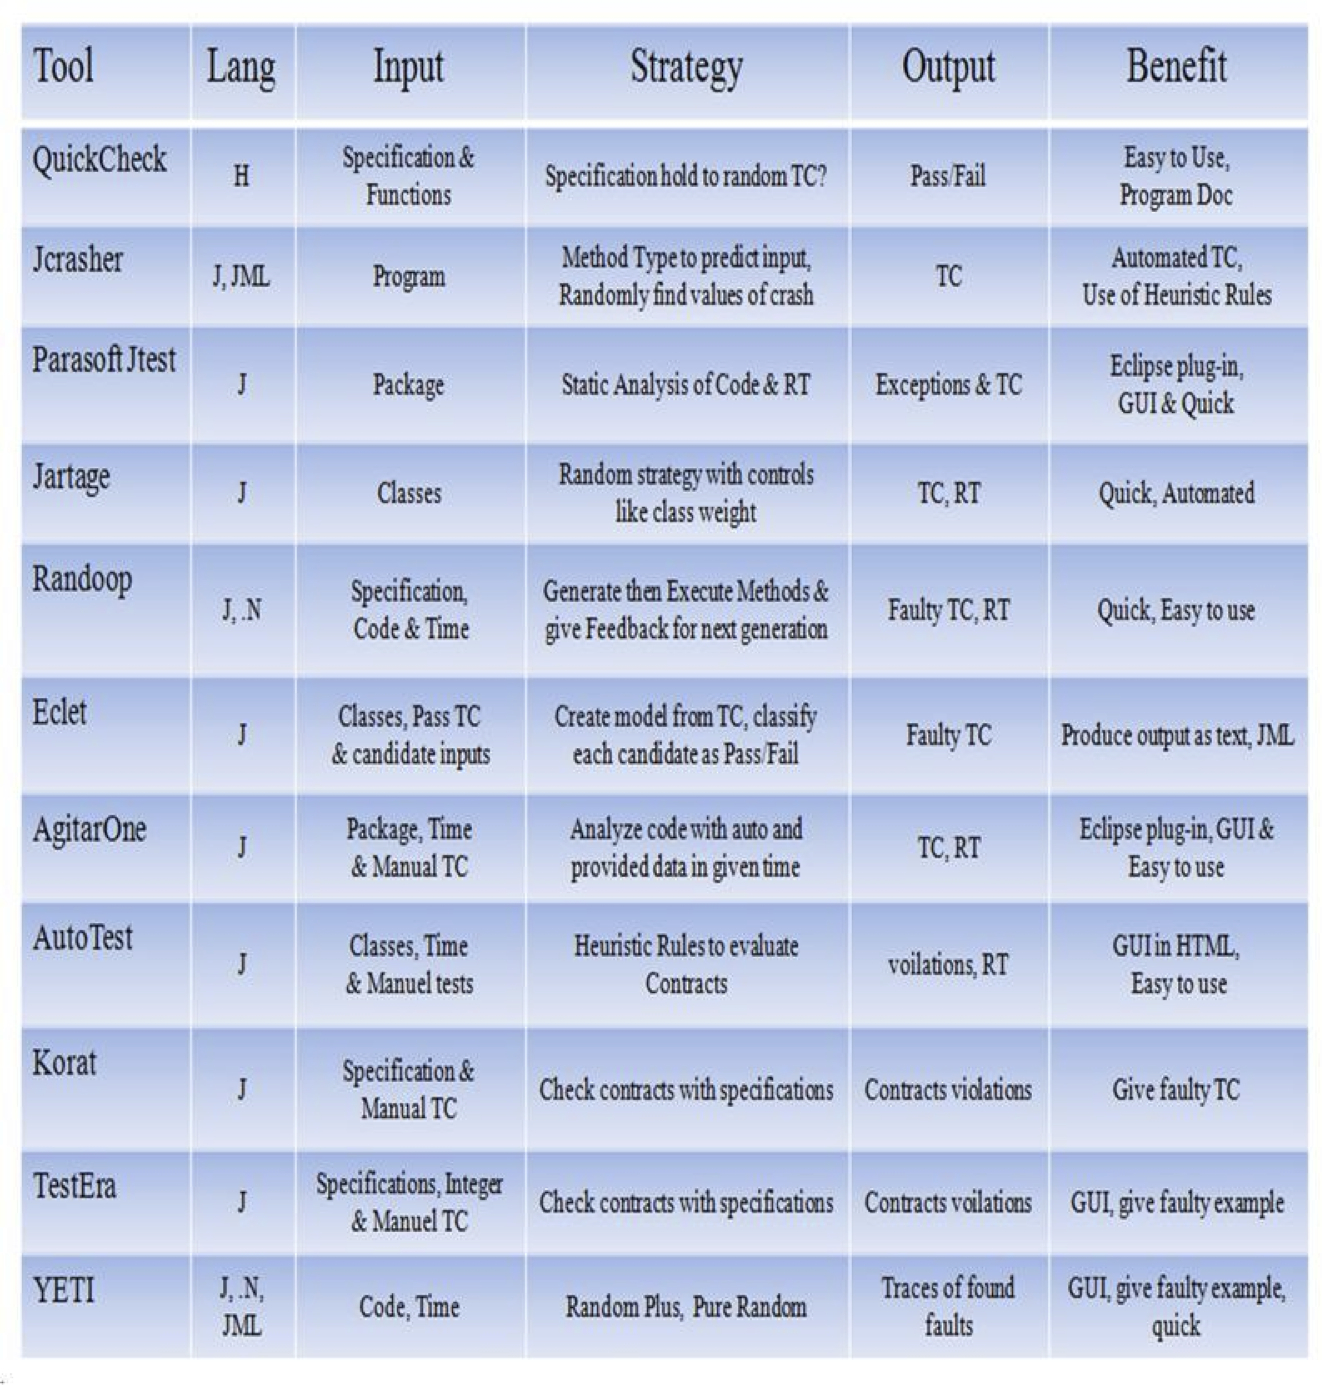
\includegraphics[scale=0.6]{chapter2/tools.jpg}
%	\caption{Summary of automated testing tools}
%\end{figure}




%\section{Conclusion}


% ------------------------------------------------------------------------


%%% Local Variables:
%%% mode: latex
%%% TeX-master: "../thesis"
%%% End:
